\documentclass{beamer}

% For more theme options:
%/usr/share/texmf/tex/latex/beamer/base/themes/theme/compatibility
\usepackage{beamerthemelined}

% this package seems to throw an error for me. -Juneki 12/6/14
%\usepackage[usenames,dvipsnames,svgnames,table]{xcolor}
\usepackage{soul}

\usepackage{algorithm}
\usepackage[noend]{algpseudocode}
\usepackage{graphicx}
\usepackage{caption}
\usepackage{subcaption}

\usepackage{tikz-dependency}

\newcommand{\eqnref}[1]{\eqref{eqn:#1}}
%\usepackage[usenames,dvipsnames,svgnames,table]{xcolor}  % allows better color names
\usepackage{todonotes}   % insert [disable] to disable all notes
\newcommand{\Note}[4][]{\todo[author=#2,color=#3,fancyline,#1]{#4}}
\newcommand{\noteJH}[2][]{\Note[#1]{JH}{blue!40}{#2}}
\newcommand{\noteJE}[2][]{\Note[#1]{JE}{green!40}{#2}}
\newcommand{\notewho}[3][]{\Note[#1]{#2}{orange!40}{#3}}  % extra arg with miscellaneous author
\newcommand{\NoteJH}[2][]{\noteJH[inline,#1]{#2}}
\newcommand{\NoteJE}[2][]{\noteJE[inline,#1]{#2}}
\newcommand{\Notewho}[3][]{\notewho[inline,#1]{#2}{#3}}  % extra arg with miscellaneous author



\begin{document}
\title{Deriving Multi-Headed Planar Dependency Parses from Link Grammar Parses}
\author{Juneki Hong, Jason Eisner}
\date{\today}
\frame{\titlepage \NoteJH{Include pictures of us?}}

\section{Motivation}
\frame{\frametitle{Motivation}
  \begin{itemize}
    \item A multiheaded dependency corpus would be useful for testing new parsing algorithms
    \item[]  
    \item[]  
    \item[]  
  \end{itemize}
}


\frame{\frametitle{Motivation}
  \begin{itemize}
    \item A multiheaded dependency corpus would be useful for testing new parsing algorithms
    \item Such a corpus could be automatically annotated using Integer Linear Programming
    \item[]  
    \item[]  
  \end{itemize}
}

\frame{\frametitle{Motivation}
  \begin{itemize}
    \item A multiheaded dependency corpus would be useful for testing new parsing algorithms
    \item Such a corpus could be automatically annotated using Integer Linear Programming
    \item We explored whether the Link Grammar could be adapted for this purpose.
    \item[]  
  \end{itemize}
}

\frame{\frametitle{Motivation}
  \begin{itemize}
    \item A multiheaded dependency corpus would be useful for testing new parsing algorithms
    \item Such a corpus could be automatically annotated using Integer Linear Programming
    \item We explored whether the Link Grammar could be adapted for this purpose.
    \item The results of this are mixed, but provides a good case study.
  \end{itemize}
}


\section{Multi-headed}

\frame{\frametitle{Multi-headedness}
  \begin{itemize}
    \item Control
    \item Relativization
    \item Conjunction
  \end{itemize}
}

\subsection{Control}
\frame{\frametitle{Control}
  \begin{figure}
    \begin{dependency}
      \begin{deptext}
        Jill \& likes \& to \& skip \\
      \end{deptext}
      \deproot[edge above, thick, hide label, edge unit distance = 1.5ex]{2}{}
      \depedge[edge above, thick, hide label]{2}{1}{}
      \depedge[edge below, ultra thick, hide label, edge style = {purple}, edge unit distance = 1.2ex]{4}{1}{}
      \depedge[edge above, thick, hide label]{2}{3}{}
      \depedge[edge above, thick, hide label]{3}{4}{}
    \end{dependency}
    \caption*{Jill is the subject of two verbs}
  \end{figure}

  \begin{figure}
    \begin{dependency}
      \begin{deptext}
        Jill \& persuaded \& Jack \& to \& skip \\
      \end{deptext}
      \deproot[edge above, thick, hide label, edge unit distance = 1.5ex]{2}{}
      \depedge[edge above, thick, hide label]{2}{1}{}
      \depedge[edge above, thick, hide label]{2}{3}{}
      \depedge[edge above, thick, hide label]{3}{4}{}
      \depedge[edge above, thick, hide label]{4}{5}{}
      \depedge[edge below, ultra thick, hide label, edge style = {purple}, edge unit distance = 1.5ex]{3}{5}{}
    \end{dependency}
    \caption*{Jack is the object of one verb and the subject of another}
  \end{figure}
}


\subsection{Relativization}
\frame{\frametitle{Relativization}
  \begin{figure}
    \begin{dependency}
      \begin{deptext}
        The \& boy \& that \& Jill \& skipped \& with \& fell \& down \\
      \end{deptext}
      \deproot[edge above, thick, hide label, edge unit distance = 2ex]{7}{}
      \depedge[edge above, thick, hide label]{2}{1}{}
      \depedge[edge above, thick, hide label]{2}{3}{}
      \depedge[edge above, thick, hide label]{3}{5}{}
      \depedge[edge above, thick, hide label]{5}{4}{}
      \depedge[edge above, thick, hide label]{5}{6}{}
      \depedge[edge above, thick, hide label, edge unit distance = 1.8ex]{7}{2}{}
      \depedge[edge above, thick, hide label]{7}{8}{}
      \depedge[edge below, ultra thick, hide label, edge style = {purple}, edge unit distance = 1.5ex]{6}{2}{}
    \end{dependency}
    \caption*{The boy is the object of \textit{with} as well as the subject of \textit{fell}.}
  \end{figure}
}


\subsection{Conjunction}
\frame{\frametitle{Conjunction}
  \begin{figure}
    \begin{dependency}
      \begin{deptext}
        Jack \& and \& Jill \& went \& up \& the \& hill \\
      \end{deptext}
      \deproot[edge above, thick, hide label, edge unit distance = 2ex]{4}{}
      \depedge[edge above, thick, hide label]{2}{1}{}
      \depedge[edge above, thick, hide label]{2}{3}{}
      \depedge[edge above, thick, hide label]{4}{2}{}
      \depedge[edge above, thick, hide label]{4}{5}{}
      \depedge[edge above, thick, hide label]{5}{7}{}
      \depedge[edge above, thick, hide label]{7}{6}{}

      \depedge[edge below, ultra thick, hide label, edge style = {purple}, edge unit distance = 1.5ex]{4}{1}{}
      \depedge[edge below, ultra thick, hide label, edge style = {purple}, edge unit distance = 1.5ex]{4}{3}{}

    \end{dependency}
    \caption*{Jack and Jill serve as the two arguments to \textit{and}, but are also subjects of \textit{went}.}
  \end{figure}
}



%\frame{\frametitle{Multi-headedness}
%  \begin{figure}
%    \begin{dependency}
%      \begin{deptext}
%      I \& think \& the \& man \& who \& you \& saw \& wants \& to \& eat \& sushi \\
%      \end{deptext}
%      \deproot[edge above, thick]{2}{ROOT}
%      \depedge[edge above, thick, hide label]{2}{1}{} % think -> I
%      \depedge[edge above, thick, hide label]{4}{3}{} % man -> the
%      \depedge[edge above, thick, hide label]{4}{5}{} % man -> who
%      \depedge[edge above, thick, hide label]{7}{6}{} % saw -> you
%      \depedge[edge above, thick, hide label]{8}{4}{} % wants -> man
%      \depedge[edge above, thick, hide label]{4}{7}{} % man -> saw
%      \depedge[edge above, thick, hide label]{2}{8}{} % think -> wants
%      \depedge[edge above, thick, hide label]{8}{10}{} % wants -> eat
%      \depedge[edge above, thick, hide label]{10}{9}{} % eat -> to
%      \depedge[edge above, thick, hide label]{10}{11}{} % eat -> sushi
%      \depedge[edge below, edge style = {purple}, hide label, edge unit distance = 1.5ex, ultra thick]{10}{4}{} % eat -> man
%    \end{dependency}
%    \caption*{Example of a Multiheaded Parse}
%  \end{figure}
%}



% Shouldn't mention non-projectivity. 
%\frame{\frametitle{Non-projectivity}
%\begin{figure}
%  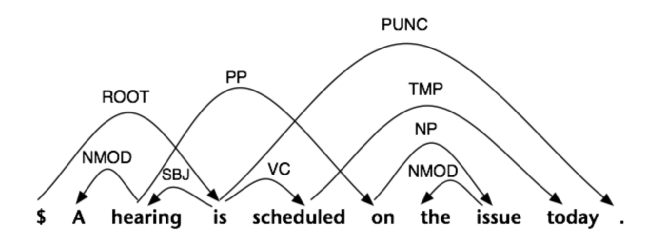
\includegraphics[width=\linewidth]{multiheaded}
%  \caption*{English is not a completely projective language}
%  \NoteJH{image taken from Chris Dyer's slide: http://demo.clab.cs.cmu.edu/fa2014-11711/images/0/0e/Depparsing.pdf}
%  \NoteJH{I should also ask Chris for permission to use this}
%\end{figure}
%}


%\section{Non Projectivity}
%\frame{\frametitle{We do not address: Non-Projectivity}
%\begin{itemize}
%  \item Projectivity assumptions allow us to have efficient parsing algorithms that utilize dynamic programming
%  \item English is mostly projective
%\end{itemize}

%\NoteJH{Should I mention non-projectivity? This slide is mostly here because of a reviewer comment.}
%}

%\frame{\frametitle{We do not address: Non-Projectivity}
%\begin{itemize}
%  \item Projectivity assumptions allow us to have efficient parsing algorithms that utilize dynamic programming
%  \item English is mostly projective
%\end{itemize}

%\begin{figure}
%  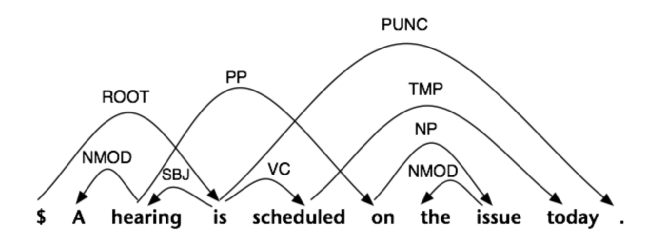
\includegraphics[width=0.7\linewidth]{multiheaded}
%  \caption*{But not always}
%  \NoteJH{image taken from Chris Dyer's slide: http://demo.clab.cs.cmu.edu/fa2014-11711/images/0/0e/Depparsing.pdf}
%  \NoteJH{I should also ask Chris for permission to use this}
%\end{figure}


%}


\section{Link Grammars}

\frame{\frametitle{Link Grammars}
  \begin{itemize}
    \item[] Grammar-based formalism for projective dependency parsing with undirected links
    %\item We set out to discover if the undirected links are actually directed relationships.
  \end{itemize}
}


\frame{\frametitle{Link Grammars: Example Parse}
\begin{figure}
  \begin{dependency}[edge style={-}]
	\begin{deptext}
	  the \& matter \& may \& never \& even \& be \& tried \& in \& court \& . \\
	  - \& n-u \& v \& e \& e \& v \& v-d \& r \& n-u \& - \\
	\end{deptext}
	\depedge[edge above, thick, edge style = {red}]{2}{3}{S}
	\depedge[edge above, thick, edge style = {red}]{3}{6}{I}
	\depedge[edge above, thick, edge style = {red}]{2}{1}{D}
	\depedge[edge above, thick, edge style = {red}]{7}{8}{MV}
	\depedge[edge above, thick, edge style = {red}]{6}{7}{P}
	\depedge[edge above, thick, edge style = {red}]{8}{9}{J}
	\deproot[edge above, thick, edge style = {red}]{2}{W}
	\deproot[edge above, thick, edge style = {red}]{7}{WV}
	\deproot[edge above, thick, edge style = {red}]{10}{X}
	\depedge[edge above, thick, edge style = {red}]{6}{4}{E}
	\depedge[edge above, thick, edge style = {red}]{6}{5}{E}
  \end{dependency}
  \caption*{Link Parse of a sentence from Penn Tree Bank}
\end{figure}


}

\frame{\frametitle{Link Grammars: Converting into a Directed Acyclic Graph}
\begin{figure}
  \begin{dependency}
	\begin{deptext}
	  the \& matter \& may \& never \& even \& be \& tried \& in \& court \& . \\
	  - \& n-u \& v \& e \& e \& v \& v-d \& r \& n-u \& - \\
	\end{deptext}
	\depedge[edge above, thick, edge style = {red}]{2}{3}{S}
	\depedge[edge above, thick, edge style = {red}]{3}{6}{I}
	\depedge[edge above, thick, edge style = {red}]{2}{1}{D}
	\depedge[edge above, thick, edge style = {red}]{7}{8}{MV}
	\depedge[edge above, thick, edge style = {red}]{6}{7}{P}
	\depedge[edge above, thick, edge style = {red}]{8}{9}{J}
	\deproot[edge above, thick, edge style = {red}]{2}{W}
	\deproot[edge above, thick, edge style = {red}]{7}{WV}
	\deproot[edge above, thick, edge style = {red}]{10}{X}
	\depedge[edge above, thick, edge style = {red}]{6}{4}{E}
	\depedge[edge above, thick, edge style = {red}]{6}{5}{E}
  \end{dependency}

  \caption*{Directionalize the edges}
\end{figure}
}


\frame{\frametitle{Link Grammars}
Compare resulting dependency parse with CoNLL 2007 shared task. 
\begin{figure}
  \begin{dependency}
	\begin{deptext}
	  {\scriptsize DT} \& {\scriptsize NN} \& {\scriptsize MD} \& {\scriptsize RB} \& {\scriptsize RB} \& {\scriptsize VB} \& {\scriptsize VB} \& {\scriptsize IN} \& {\scriptsize NN} \& {\scriptsize .} \\
	  the \& matter \& may \& never \& even \& be \& tried \& in \& court \& . \\
	  - \& n-u \& v \& e \& e \& v \& v-d \& r \& n-u \& - \\
	\end{deptext}
	\deproot[edge above, thick, edge style = {blue}]{3}{\small ROOT}
	\depedge[edge below, thick, edge style = {red}]{2}{3}{S}
	\depedge[edge above, thick, edge style = {blue}]{3}{2}{\small SBJ}
	\depedge[edge above, thick, edge style = {blue}]{3}{4}{\small ADV}
	\depedge[edge above, thick, edge style = {blue}]{3}{5}{\small ADV}
	\depedge[edge below, thick, edge style = {red}]{3}{6}{I}
	\depedge[edge above, thick, edge style = {blue}]{3}{6}{\small VC}
	\depedge[edge above, thick, edge style = {blue}, edge unit distance =1.5ex]{3}{10}{\small P}
	\depedge[edge below, thick, edge style = {red}]{2}{1}{D}
	\depedge[edge above, thick, edge style = {blue}]{2}{1}{\small NMOD}
	\depedge[edge below, thick, edge style = {red}]{7}{8}{MV}
	\depedge[edge above, thick, edge style = {blue}]{7}{8}{\small ADV}
	\depedge[edge below, thick, edge style = {red}]{6}{7}{P}
	\depedge[edge above, thick, edge style = {blue}]{6}{7}{\small VC}
	\depedge[edge below, thick, edge style = {red}]{8}{9}{J}
	\depedge[edge above, thick, edge style = {blue}]{8}{9}{\small PMOD}
	\deproot[edge below, thick, edge style = {red}]{2}{W}
	\deproot[edge below, thick, edge style = {red}]{7}{WV}
	\deproot[edge below, thick, edge style = {red}]{10}{X}
	\depedge[edge below, thick, edge style = {red}]{6}{4}{E}
	\depedge[edge below, thick, edge style = {red}]{6}{5}{E}
  \end{dependency}

  \caption*{Top half is CoNLL. Bottom half is the directionalized link parse.}
\end{figure}


}



\frame{\frametitle{Link Grammars}
Compare resulting dependency parse with CoNLL 2007 shared task. 
\begin{figure}
  \begin{dependency}
	\begin{deptext}
	  {\scriptsize DT} \& {\scriptsize NN} \& {\scriptsize MD} \& {\scriptsize RB} \& {\scriptsize RB} \& {\scriptsize VB} \& {\scriptsize VB} \& {\scriptsize IN} \& {\scriptsize NN} \& {\scriptsize .} \\
	  the \& matter \& may \& never \& even \& be \& tried \& in \& court \& . \\
	  - \& n-u \& v \& e \& e \& v \& v-d \& r \& n-u \& - \\
	\end{deptext}
	\deproot[edge above, edge style = {blue, dotted}]{3}{\small ROOT}
	\depedge[edge below, edge style = {red, ultra thick}]{2}{3}{S}
	\depedge[edge above, edge style = {blue, ultra thick}]{3}{2}{\small SBJ}
	\depedge[edge above, edge style = {blue, dotted}]{3}{4}{\small ADV}
	\depedge[edge above, edge style = {blue, dotted}]{3}{5}{\small ADV}
	\depedge[edge below, edge style = {red, thick}]{3}{6}{I}
	\depedge[edge above, edge style = {blue, thick}]{3}{6}{\small VC}
	\depedge[edge above, edge style = {blue, dotted}, edge unit distance =1.5ex]{3}{10}{\small P}
	\depedge[edge below, edge style = {red, thick}]{2}{1}{D}
	\depedge[edge above, edge style = {blue, thick}]{2}{1}{\small NMOD}
	\depedge[edge below, edge style = {red, thick}]{7}{8}{MV}
	\depedge[edge above, edge style = {blue, thick}]{7}{8}{\small ADV}
	\depedge[edge below, edge style = {orange, thick}]{6}{7}{P}
	\depedge[edge above, edge style = {blue, thick}]{6}{7}{\small VC}
	\depedge[edge below, edge style = {red, thick}]{8}{9}{J}
	\depedge[edge above, edge style = {blue, thick}]{8}{9}{\small PMOD}
	\deproot[edge below, edge style = {red, dotted}]{2}{W}
	\deproot[edge below, edge style = {orange, ultra thick, dotted}]{7}{WV}
	\deproot[edge below, edge style = {red, dotted}]{10}{X}
	\depedge[edge below, edge style = {red, dotted}]{6}{4}{E}
	\depedge[edge below, edge style = {red, dotted}]{6}{5}{E}
  \end{dependency}

  \caption*{Top half is CoNLL. Bottom half is the directionalized link parse.}
\end{figure}


}


%\section{ILP}
%\frame{\frametitle{Integer Linear Programming}

%\NoteJH{Will the audience know about ILP?}

%}


\section{ILP Model}


\frame{\frametitle{Integer Linear Programming Model}

Encoded Constraints:
\begin{itemize}
  \item Connectedness
  \item Acyclicity
  \item Consistency of Directionalized Links
\end{itemize}
}



\frame{\frametitle{Integer Linear Programming Model}

For each sentence, for each edge $i,j$, where $i < j$

\begin{figure}
  \begin{dependency}[edge style={-}]
    \begin{deptext}
      . \& . \& . \& $i$ \& . \& . \& . \& $j$ \& . \& . \& . \\
    \end{deptext}
    \depedge[edge above, thick, edge unit distance = 1.1ex]{4}{8}{L}
  \end{dependency}
\end{figure}



Variables: 
\begin{itemize}
\item[] $x_{ij}, x_{ji} \in \mathbb{Z} \geq 0$: orientation of each link
\item[] $x_{ij} + x_{ji} = 1$

%\item $x_{ij} + x_{ji} = 1$ (A link can only be oriented left or right)

\end{itemize}





%\NoteJH{TODO: Incomplete slide. Need to describe things like depth of the variable, label}
}



\frame{\frametitle{Connectedness, Acyclicity}
\begin{itemize}
  \item[] Connectedness
    \begin{align}
      \sum_u x_{uv} & \geq 1
    \end{align}

  \item[] Acyclicity
    \begin{itemize}
      \item[] Given that node $u$ is the parent of $v$
      \item[] $n_v$: length of the sentence containing node $v$
      \item[] $d_v \in [0, n_v]$: depth of the node from the root of the sentence
    \end{itemize}

    \begin{align}
      (\forall_u)\; d_v + (1 + n_v) \cdot (1 - x_{uv}) & \geq 1+d_u
    \end{align}
\end{itemize}

}


\frame{\frametitle{Consistency of Directionalized Links}
\begin{itemize}
  \item[] Consistency of Directionalized Links
    \begin{itemize}
      \item[] $r_L, \ell_L \in \{0,1\}$: whether links with label $L$ allowed left/right
    \end{itemize}
    \begin{align}\label{direction+slack}
      x_{ij} &\leq r_L &
      x_{ji} &\leq \ell_L 
    \end{align}
    \begin{align}\label{eqn:obj}
      \min \left( \sum_L r_L + \ell_L \right)
    \end{align}
    \begin{itemize}
      \item[]  
      \item[]  
    \end{itemize}

    \begin{itemize}
      \item[]
    \end{itemize}

\end{itemize}
}

\frame{\frametitle{Consistency of Directionalized Links with Slack}
\begin{itemize}
  \item[] Consistency of Directionalized Links
    \begin{itemize}
      \item[] $r_L, \ell_L \in \{0,1\}$: whether links with label $L$ allowed left/right
    \end{itemize}
    \begin{align}\label{direction+slack}
      x_{ij} &\leq r_L + s_{ij} &
      x_{ji} &\leq \ell_L + s_{ij} 
    \end{align}
    \begin{align}\label{eqn:obj}
      \min \left( \sum_L r_L + \ell_L \right) \cdot \frac{N_L}{4} + \sum_{ij}s_{ij}
    \end{align}
    \begin{itemize}
      \item[] $s_{ij} \in \mathbb{R} \geq 0$: slack variable 
      \item[] $N_L$: Number of link tokens with label $L$
    \end{itemize}

    \begin{itemize}
      \item[] Slack allows a few links with label $L$ in disallowed directions
    \end{itemize}

\end{itemize}
}






\section{Experiments and Results}
%\frame{\frametitle{Experiments and Results}
%\begin{itemize}
%  \item 18,577 English sentences with gold CoNLL. 
%  \item 18,577 unlabeled Russian sentences.
%\end{itemize}
%}

\frame{\frametitle{Data Sets}
%\begin{itemize}
%  \item[] 18,577 English sentences with 10,960 connected parses
%  \item[] 18,577 unlabeled Russian sentences with 4,913 connected parses
%\end{itemize}
  \begin{table}[h]
    \begin{tabular}{|l|l|l|}
      \hline
      & \# Sentences & \# Connected Parses \\ \hline
      English             & 18,577        & 10,960               \\ \hline
      Russian (unlabeled) & 18,577        & 4,913                \\ \hline
    \end{tabular}
  \end{table}
  
  On the English data set:
  
  \begin{itemize}
  \item[] Link Data has 8\% additional edges over the CoNLL.
  \item[] 52\% of links match CoNLL arcs
  \item[] 57\% of CoNLL arcs match links
  \end{itemize}
  
  \NoteJH{I skipped the ``Stability of Results'' section}
}

%\frame{\frametitle{On the English data set}
%\begin{itemize}
%\item[] Link Data has 8\% additional edges over the CoNLL.
%\item[] 52\% of links match CoNLL arcs
%\item[] 57\% of CoNLL arcs match links
%\end{itemize}

%
%}

\frame{\frametitle{ILP Results}
%  \begin{table}[h]
%    \begin{tabular}{|l|l||l|}
%      \hline
%      & & out of total \\ \hline
%      Link types & & \\allowing both directions & 7 & 113 \\ \hline
%      Link tokens & & \\requiring disallowed direction & & \\via slack & 4043 & 195,000 \\ \hline
%    \end{tabular}
%  \end{table}
  \begin{itemize}
  \item[] Link types that allowed both directions:
    \begin{itemize}
    \item[] 7 / 113 = 6.19\%
    \end{itemize}
  \item[] Link tokens that required disallowed direction via slack:
    \begin{itemize}
    \item[] 4043 / 195,000 = 2.07\%
    \end{itemize}
  \end{itemize}
  \begin{itemize}
  \item[]  
  \end{itemize}
}

\frame{\frametitle{ILP Results}
  \begin{itemize}
    \item[] Link types that allowed both directions:
      \begin{itemize}
      \item[] 7 / 113 = 6.19\%
      %\item[] $\frac{7}{113} = 6.19\%$ 
      \end{itemize}
    \item[] Link tokens that required disallowed direction via slack:
      \begin{itemize}
        %\item[] $\frac{4043}{195000} = 2.07\%$ 
        \item[] 4043 / 195,000 = 2.07\%
      \end{itemize}
  \end{itemize}
  \begin{itemize}
  \item[] The link labels mostly have a consistent direction.
  \end{itemize}
}




\frame{\frametitle{Link Results: Subject-Verb links are backwards}
\begin{figure}
  \begin{dependency}
	\begin{deptext}
	  {\scriptsize DT} \& {\scriptsize NN} \& {\scriptsize MD} \& {\scriptsize RB} \& {\scriptsize RB} \& {\scriptsize VB} \& {\scriptsize VB} \& {\scriptsize IN} \& {\scriptsize NN} \& {\scriptsize .} \\
	  the \& matter \& may \& never \& even \& be \& tried \& in \& court \& . \\
	  - \& n-u \& v \& e \& e \& v \& v-d \& r \& n-u \& - \\
	\end{deptext}
	\deproot[edge above, edge style = {blue, dotted}]{3}{\small ROOT}
	\depedge[edge below, edge style = {red, ultra thick}]{2}{3}{S}
	\depedge[edge above, edge style = {blue, ultra thick}]{3}{2}{\small SBJ}
	\depedge[edge above, edge style = {blue, dotted}]{3}{4}{\small ADV}
	\depedge[edge above, edge style = {blue, dotted}]{3}{5}{\small ADV}
	\depedge[edge below, edge style = {red, thick}]{3}{6}{I}
	\depedge[edge above, edge style = {blue, thick}]{3}{6}{\small VC}
	\depedge[edge above, edge style = {blue, dotted}, edge unit distance =1.5ex]{3}{10}{\small P}
	\depedge[edge below, edge style = {red, thick}]{2}{1}{D}
	\depedge[edge above, edge style = {blue, thick}]{2}{1}{\small NMOD}
	\depedge[edge below, edge style = {red, thick}]{7}{8}{MV}
	\depedge[edge above, edge style = {blue, thick}]{7}{8}{\small ADV}
	\depedge[edge below, edge style = {orange, thick}]{6}{7}{P}
	\depedge[edge above, edge style = {blue, thick}]{6}{7}{\small VC}
	\depedge[edge below, edge style = {red, thick}]{8}{9}{J}
	\depedge[edge above, edge style = {blue, thick}]{8}{9}{\small PMOD}
	\deproot[edge below, edge style = {red, dotted}]{2}{W}
	\deproot[edge below, edge style = {orange, ultra thick, dotted}]{7}{WV}
	\deproot[edge below, edge style = {red, dotted}]{10}{X}
	\depedge[edge below, edge style = {red, dotted}]{6}{4}{E}
	\depedge[edge below, edge style = {red, dotted}]{6}{5}{E}
  \end{dependency}
\end{figure}

\begin{itemize}
\item[] %This is probably due to an inconsistency of the Link Grammar, discovered by our method.
\end{itemize}

}



\frame{\frametitle{Link Results: Subject-Verb links are backwards}
\begin{figure}
  \begin{dependency}
	\begin{deptext}
	  {\scriptsize DT} \& {\scriptsize NN} \& {\scriptsize MD} \& {\scriptsize RB} \& {\scriptsize RB} \& {\scriptsize VB} \& {\scriptsize VB} \& {\scriptsize IN} \& {\scriptsize NN} \& {\scriptsize .} \\
	  the \& matter \& may \& never \& even \& be \& tried \& in \& court \& . \\
	  - \& n-u \& v \& e \& e \& v \& v-d \& r \& n-u \& - \\
	\end{deptext}
	\deproot[edge above, edge style = {gray}, hide label]{3}{\small ROOT}
	\depedge[edge below, edge style = {red, ultra thick}]{2}{3}{S}
	\depedge[edge above, edge style = {blue, ultra thick}]{3}{2}{\small SBJ}
	\depedge[edge above, edge style = {gray}, hide label]{3}{4}{\small ADV}
	\depedge[edge above, edge style = {gray}, hide label]{3}{5}{\small ADV}
	\depedge[edge below, edge style = {gray}, hide label]{3}{6}{I}
	\depedge[edge above, edge style = {gray}, hide label]{3}{6}{\small VC}
	\depedge[edge above, , edge style = {gray}, hide label, edge unit distance =1.5ex]{3}{10}{\small P}
	\depedge[edge below, edge style = {gray}, hide label]{2}{1}{D}
	\depedge[edge above, edge style = {gray}, hide label]{2}{1}{\small NMOD}
	\depedge[edge below, edge style = {gray}, hide label]{7}{8}{MV}
    \depedge[edge above, edge style = {gray}, hide label]{7}{8}{\small ADV}
	\depedge[edge below, edge style = {gray}, hide label]{6}{7}{P}
	\depedge[edge above, edge style = {gray}, hide label]{6}{7}{\small VC}
	\depedge[edge below, edge style = {gray}, hide label]{8}{9}{J}
	\depedge[edge above, edge style = {gray}, hide label]{8}{9}{\small PMOD}
	\deproot[edge below, edge style = {gray}, hide label]{2}{W}
    \deproot[edge below, edge style = {gray}, hide label]{7}{WV}
	\deproot[edge below, edge style = {gray}, hide label]{10}{X}
	\depedge[edge below, edge style = {gray}, hide label]{6}{4}{E}
	\depedge[edge below, edge style = {gray}, hide label]{6}{5}{E}
  \end{dependency}
\end{figure}

\begin{itemize}
\item This is due to an inconsistency of the Link Grammar, discovered by our method. 
\end{itemize}

\NoteJH{Should I include a section of the appendix table? Which rows should I include?}
}


\section{Conclusions}
\frame{\frametitle{Conclusions}
  \begin{itemize}
  \item Link Grammar parses can be oriented into connected DAGs
  \item New corpora for building multi-headed dependency parsers
  \item ILP can be used to build or annotate corpora
  \end{itemize}
}


\frame{\frametitle{}
  \begin{itemize}
  \item[] Questions?
  \end{itemize}
}



%\nocite{*}
%\bibliographystyle{plain}
%\bibliography{hong+eisner.TLT13.slides.bib}
%\appendix

\end{document}
